\setbeamercolor{background canvas}{bg=fitblue}
\begin{frame}
  \frametitle{Procedurální generování}
  \begin{center}
    \Huge {\color{white}Procedurální generování}
  \end{center}
\end{frame}
\setbeamercolor{background canvas}{bg=white}

\begin{frame}
\frametitle{Procedurální generování}
	\begin{itemize}
	\item{Neukládáme data grafických objektů.}
	\item{Neukládáme vrcholy, pixely, barvy, ...}
	\item{Ukládáme šablony a způsob vygenerování grafického objektu.}
	\item{Uložení algoritmu pro vygenerování zabírá pár kB.}
	\item{Uložení v textovém souboru - parametry.}
	\item{Můžeme generovat i šablony.}
	\item{Málo místa pro uložení vs doba generování.}
	\end{itemize}
\end{frame}

\begin{frame}
\frametitle{Fraktály}
	\begin{figure}[h]
		
\includegraphics[width=10cm,keepaspectratio]{pics/procedural/fractal.jpg}
	\end{figure}
\end{frame}

\begin{frame}
\frametitle{Fraktály}
	\begin{figure}[h]
		
\includegraphics[width=2.8cm,keepaspectratio]{pics/procedural/weed0.jpg}
		
\includegraphics[width=2.8cm,keepaspectratio]{pics/procedural/weed1.jpg}
		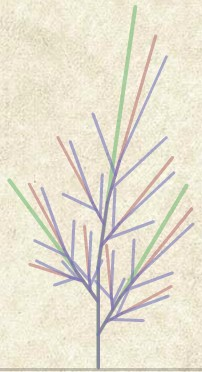
\includegraphics[width=2.8cm,keepaspectratio]{pics/procedural/weed2.jpg}
		
\includegraphics[width=2.8cm,keepaspectratio]{pics/procedural/weed3.jpg}
	\end{figure}
	\url{http://www.dangries.com/Flash/FractalMakerExp/FractalMaker_exp.html}
\end{frame}

\begin{frame}
\frametitle{L-systém}
	\begin{figure}[h]
		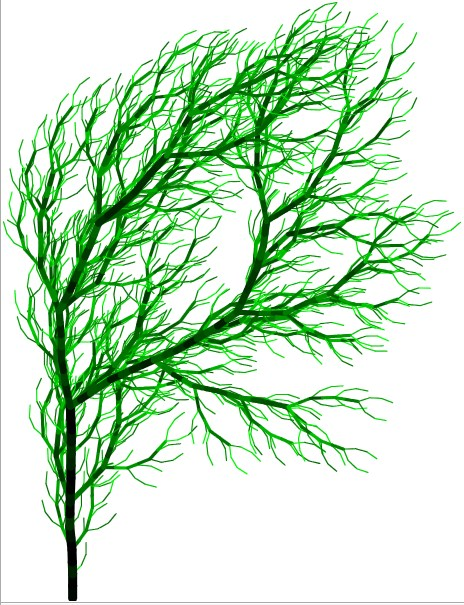
\includegraphics[width=4cm,keepaspectratio]{pics/procedural/lsystem.jpg}
		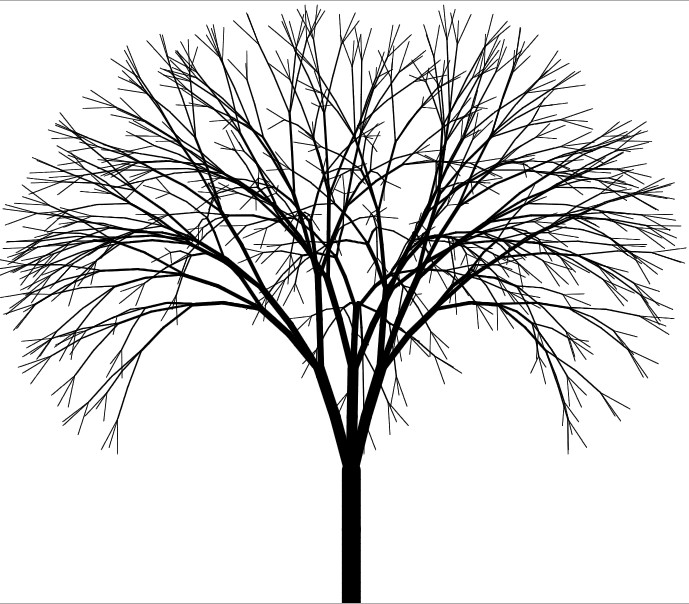
\includegraphics[width=4cm,keepaspectratio]{pics/procedural/lsystem1.jpg}
	\end{figure}
	\url{http://malsys.cz/}
\end{frame}

\begin{frame}
\frametitle{L-systém}
	\begin{figure}[h]
		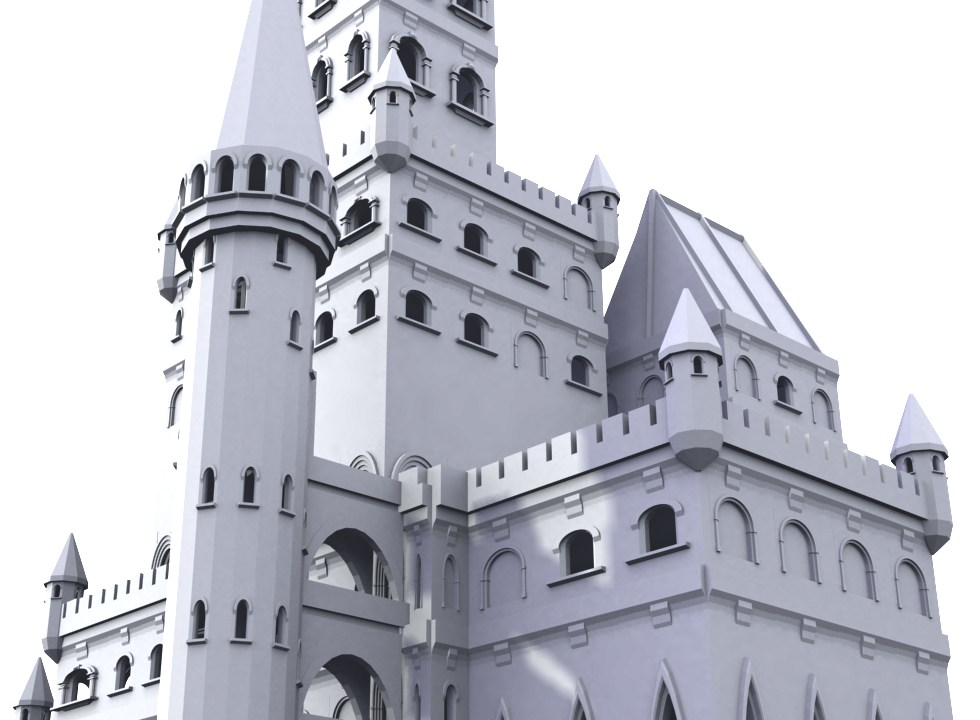
\includegraphics[width=10cm,keepaspectratio]{pics/procedural/castle.jpg}
	\end{figure}
	\url{http://procworld.blogspot.com/}
\end{frame}

\begin{frame}
\frametitle{Šumy a voroného diagramy}
	\begin{itemize}
		\item Perlin/Simple noise
    \item Voroného diagramy
	\end{itemize}
	\begin{figure}[h]
		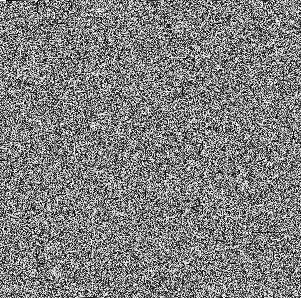
\includegraphics[width=3cm,keepaspectratio]{pics/procedural/simple_noise}
		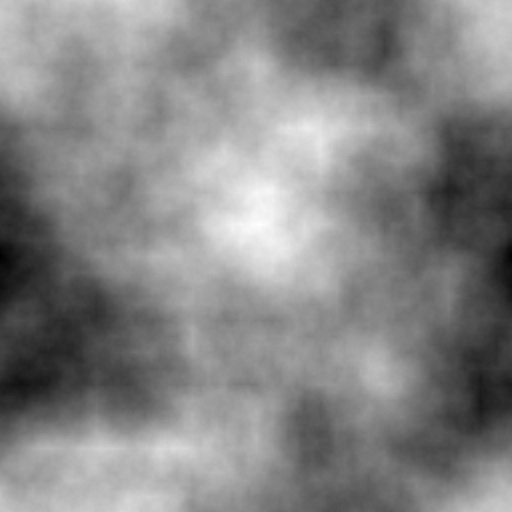
\includegraphics[width=3cm,keepaspectratio]{pics/procedural/midpoint_noise}
		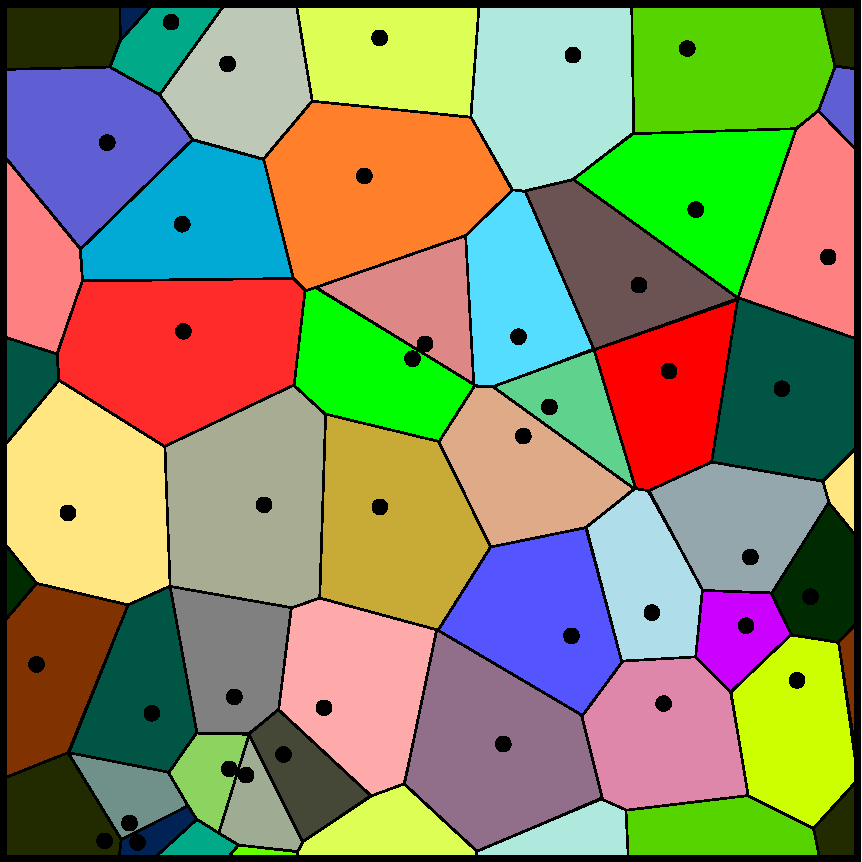
\includegraphics[width=3cm,keepaspectratio]{pics/procedural/voronoid}
	\end{figure}
\end{frame}


\begin{frame}
\frametitle{Textury založené na šumech}
	\begin{figure}[h]
		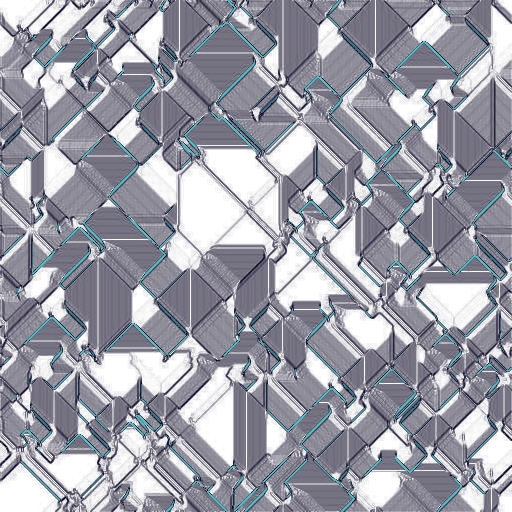
\includegraphics[width=3cm,keepaspectratio]{pics/procedural/tex00.jpg}
		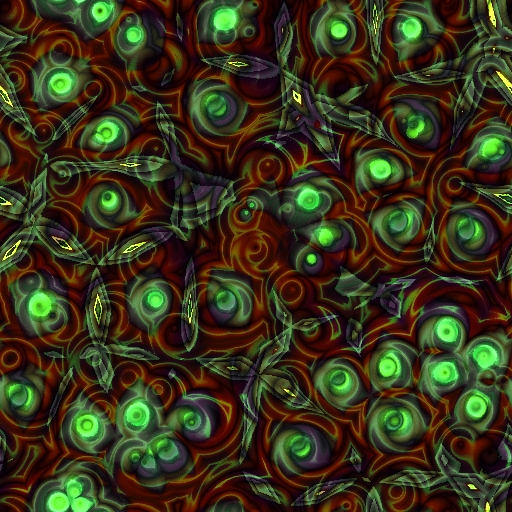
\includegraphics[width=3cm,keepaspectratio]{pics/procedural/tex01.jpg}
		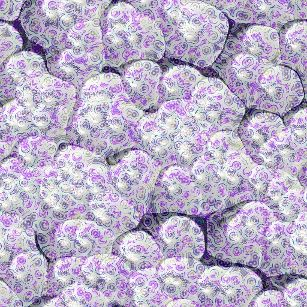
\includegraphics[width=3cm,keepaspectratio]{pics/procedural/tex02.jpg}
	\end{figure}
\end{frame}

\begin{frame}
    \frametitle{Procedurální textury}

    \begin{columns}[c]
    \column{.5\textwidth}
        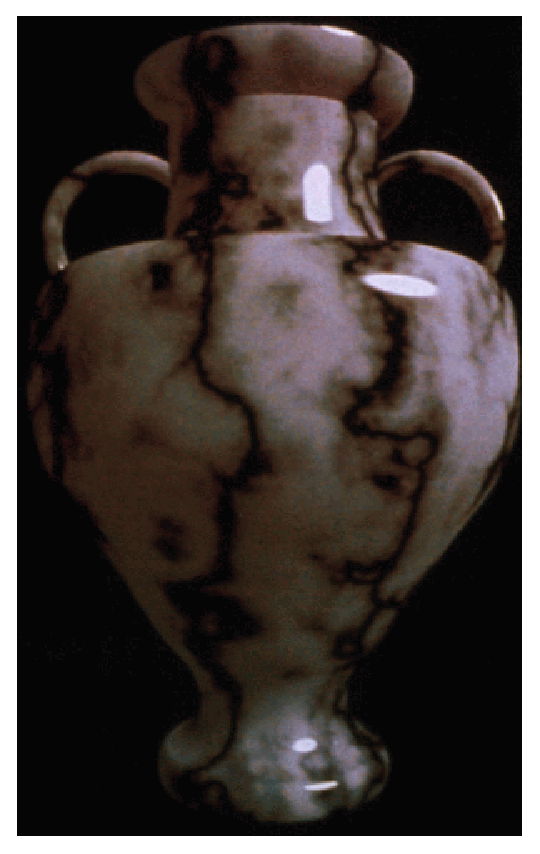
\includegraphics[width=\textwidth]{pics/procedural/vase.eps}
    \column{.5\textwidth}
        \begin{itemize}
            \item Výpočet hodnoty v shaderu.
            \item Málo paměti.
            \item Neomezené rozlišení.
            \item Vhodné pro dema.
            \item Šum
        \end{itemize}
    \end{columns}
\end{frame}

\begin{frame}
    \frametitle{Šum v grafice}
    Chceme šumové funkce
    \begin{itemize}
        \item float noise(float p)
        \item float noise(vec2 p)
        \item ...
    \end{itemize}
    \vfill
    \begin{itemize}
        \item Pseudonáhodné
        \item Výstup v $[0,1]$ nebo $[-1,1]$
        \item Deterministické
        \item Omezené frekvenční spektrum
    \end{itemize}
\end{frame}

\begin{frame}[fragile]
    \frametitle{Hodnotový šum}
    \begin{columns}[c]
    \column{.5\textwidth}
        \begin{itemize}
            \item Náhodně vygenerovaná textura.
            \item Rychle se opakuje.
            \item Interpolaci a opakování zařídí OpenGL.
        \end{itemize}
    \column{.5\textwidth}
        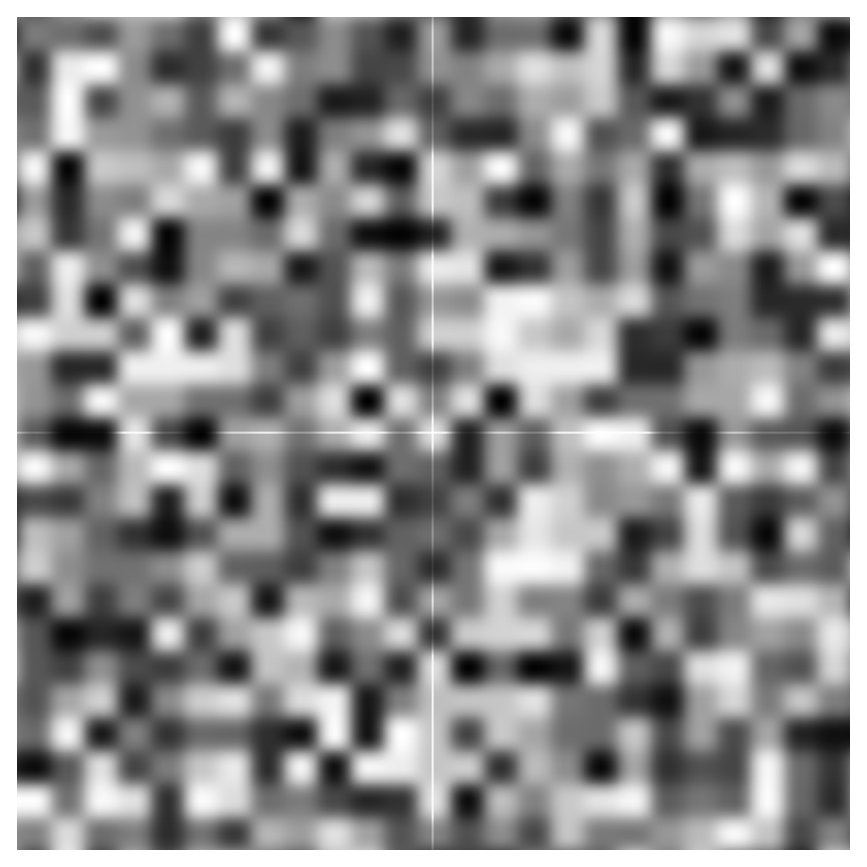
\includegraphics[width=\textwidth]{pics/procedural/value_noise.eps}
    \end{columns}

  \begin{minted}[frame=lines]{glsl}
float noise(vec2 p)
{
    return 2*texture(noiseTexture, p).x - 1;
}
  \end{minted}
\end{frame}

\begin{frame}[fragile]
    \frametitle{Gradientní šum}
    \begin{columns}[c]
    \column{.5\textwidth}
        \begin{itemize}
            \item V textuře jsou \textbf{gradienty}.
            \item Spočítáme si směrové vektory od \textbf{texelů} ke \textbf{vzorku}.
            \item Skalární součin směrů s gradienty dává výsledný šum.
        \end{itemize}
        
\includegraphics[width=.5\textwidth]{pics/procedural/grad_noise.eps}
    \column{.5\textwidth}
        
\includegraphics[width=\textwidth]{pics/procedural/perlin_noise.eps}
    \end{columns}
    Perlin K.; Implementing Improved Perlin Noise, GPU Gems\\
    Green S.; Implementing Improved Perlin Noise, GPU Gems 2
\end{frame}

\begin{frame}[fragile]
    \frametitle{Fraktální šum}
    \begin{columns}[c]
    \column{.5\textwidth}
        \begin{itemize}
            \item Sčítáme vrstvy o různé frekvenci a amplitudě
            \item Oktávy
        \end{itemize}
    \column{.5\textwidth}
        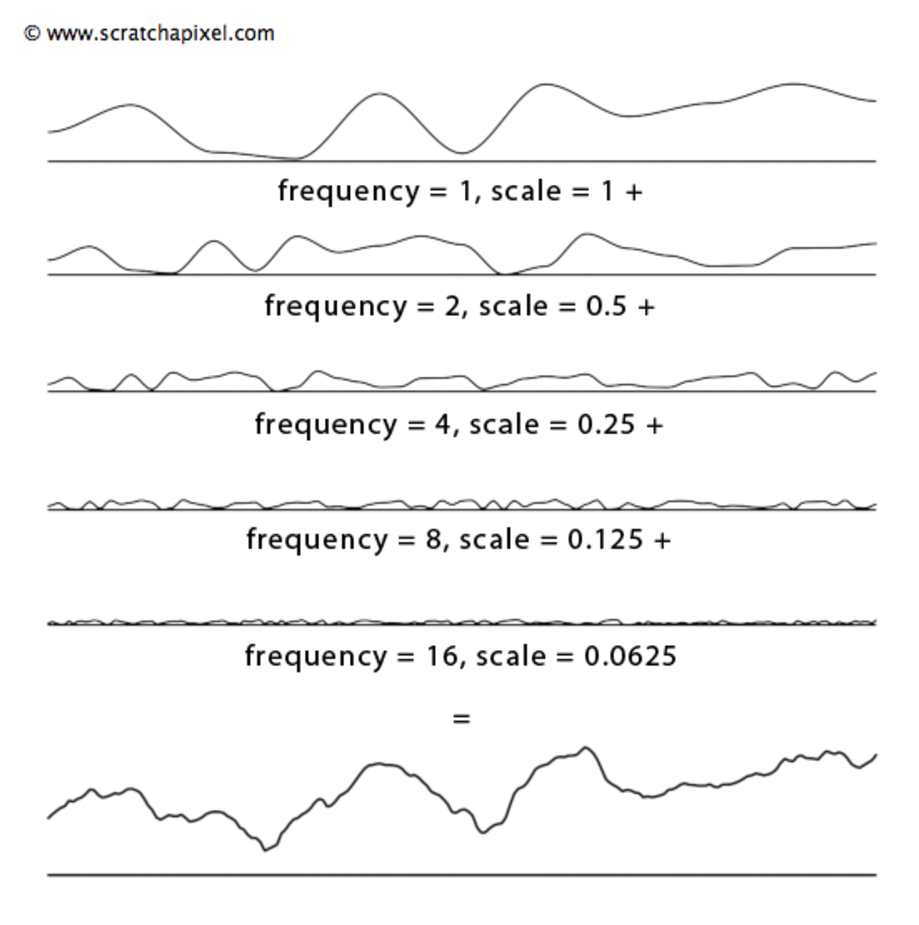
\includegraphics[width=\textwidth]{pics/procedural/1dnoise-fractal.eps}
    \end{columns}
  \begin{minted}[frame=lines]{glsl}
float fnoise(vec2 p)
{
    return noise(p)
        + 0.5*noise(2*p)
        + 0.25*noise(4*p);
}
  \end{minted}
\end{frame}

\begin{frame}
    \frametitle{Výsledek}
    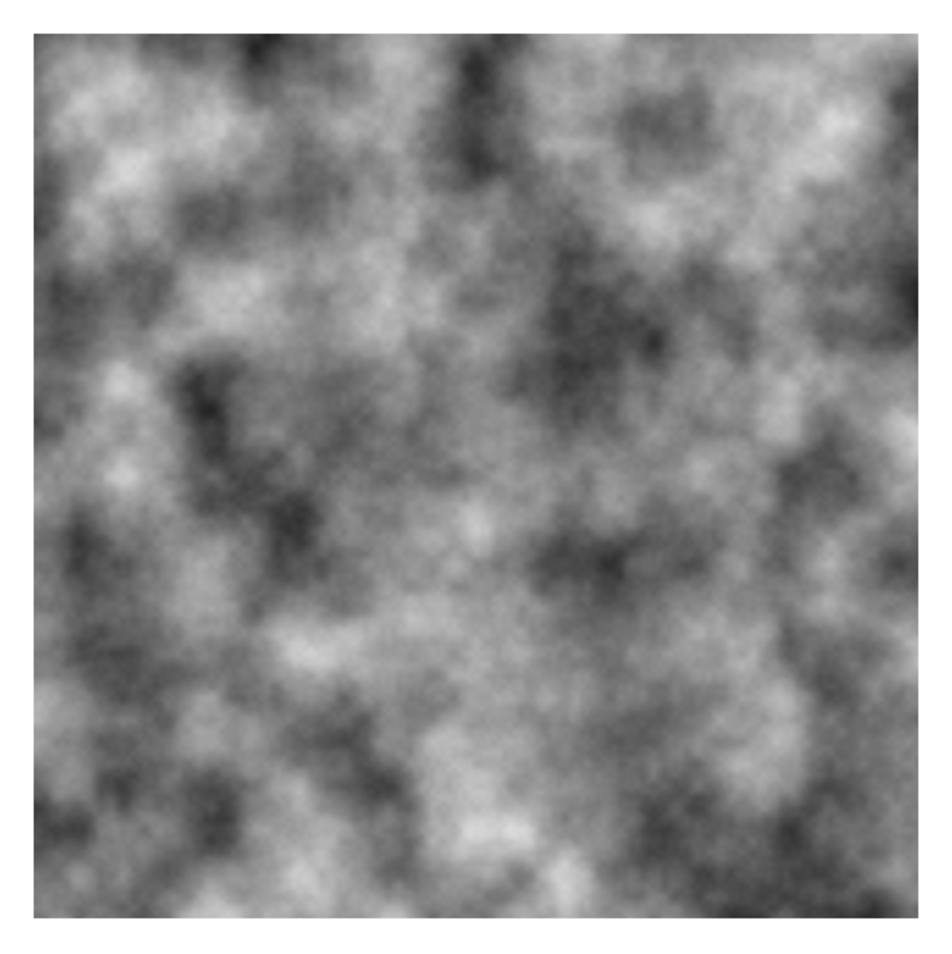
\includegraphics[width=\textwidth]{pics/procedural/2dnoise-fractal.eps}
\end{frame}

\begin{frame}
    \frametitle{Jednoduchý priklad}
    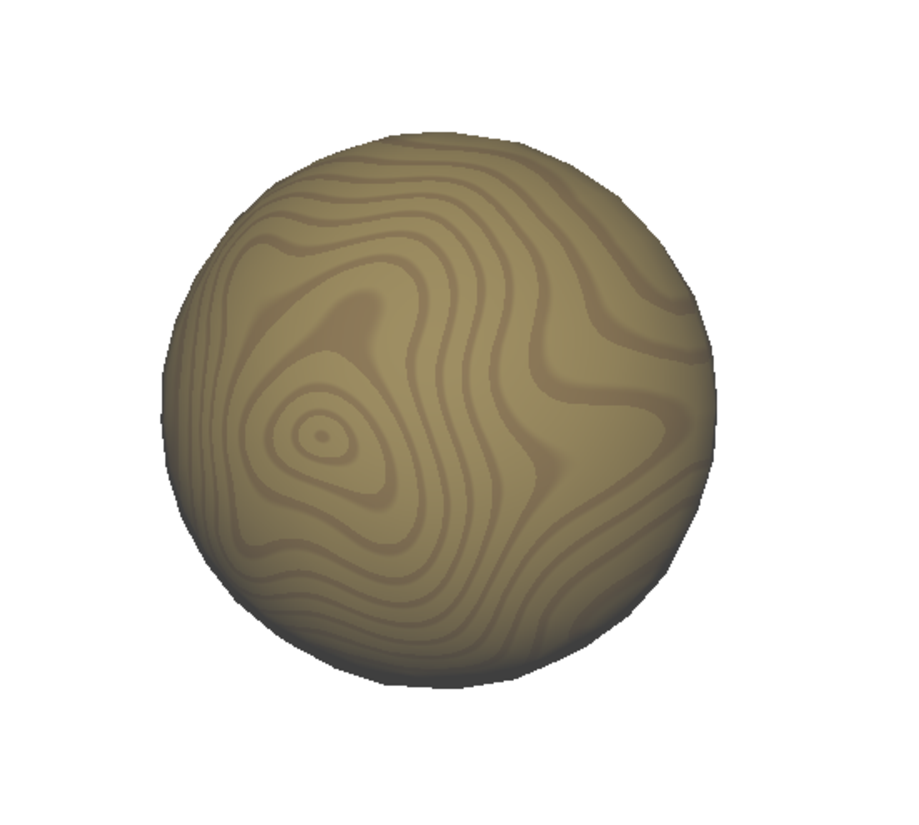
\includegraphics[width=\textwidth]{pics/procedural/drevo.eps}
\end{frame}
 
\begin{frame}[fragile]
    \frametitle{Letokruhy}
    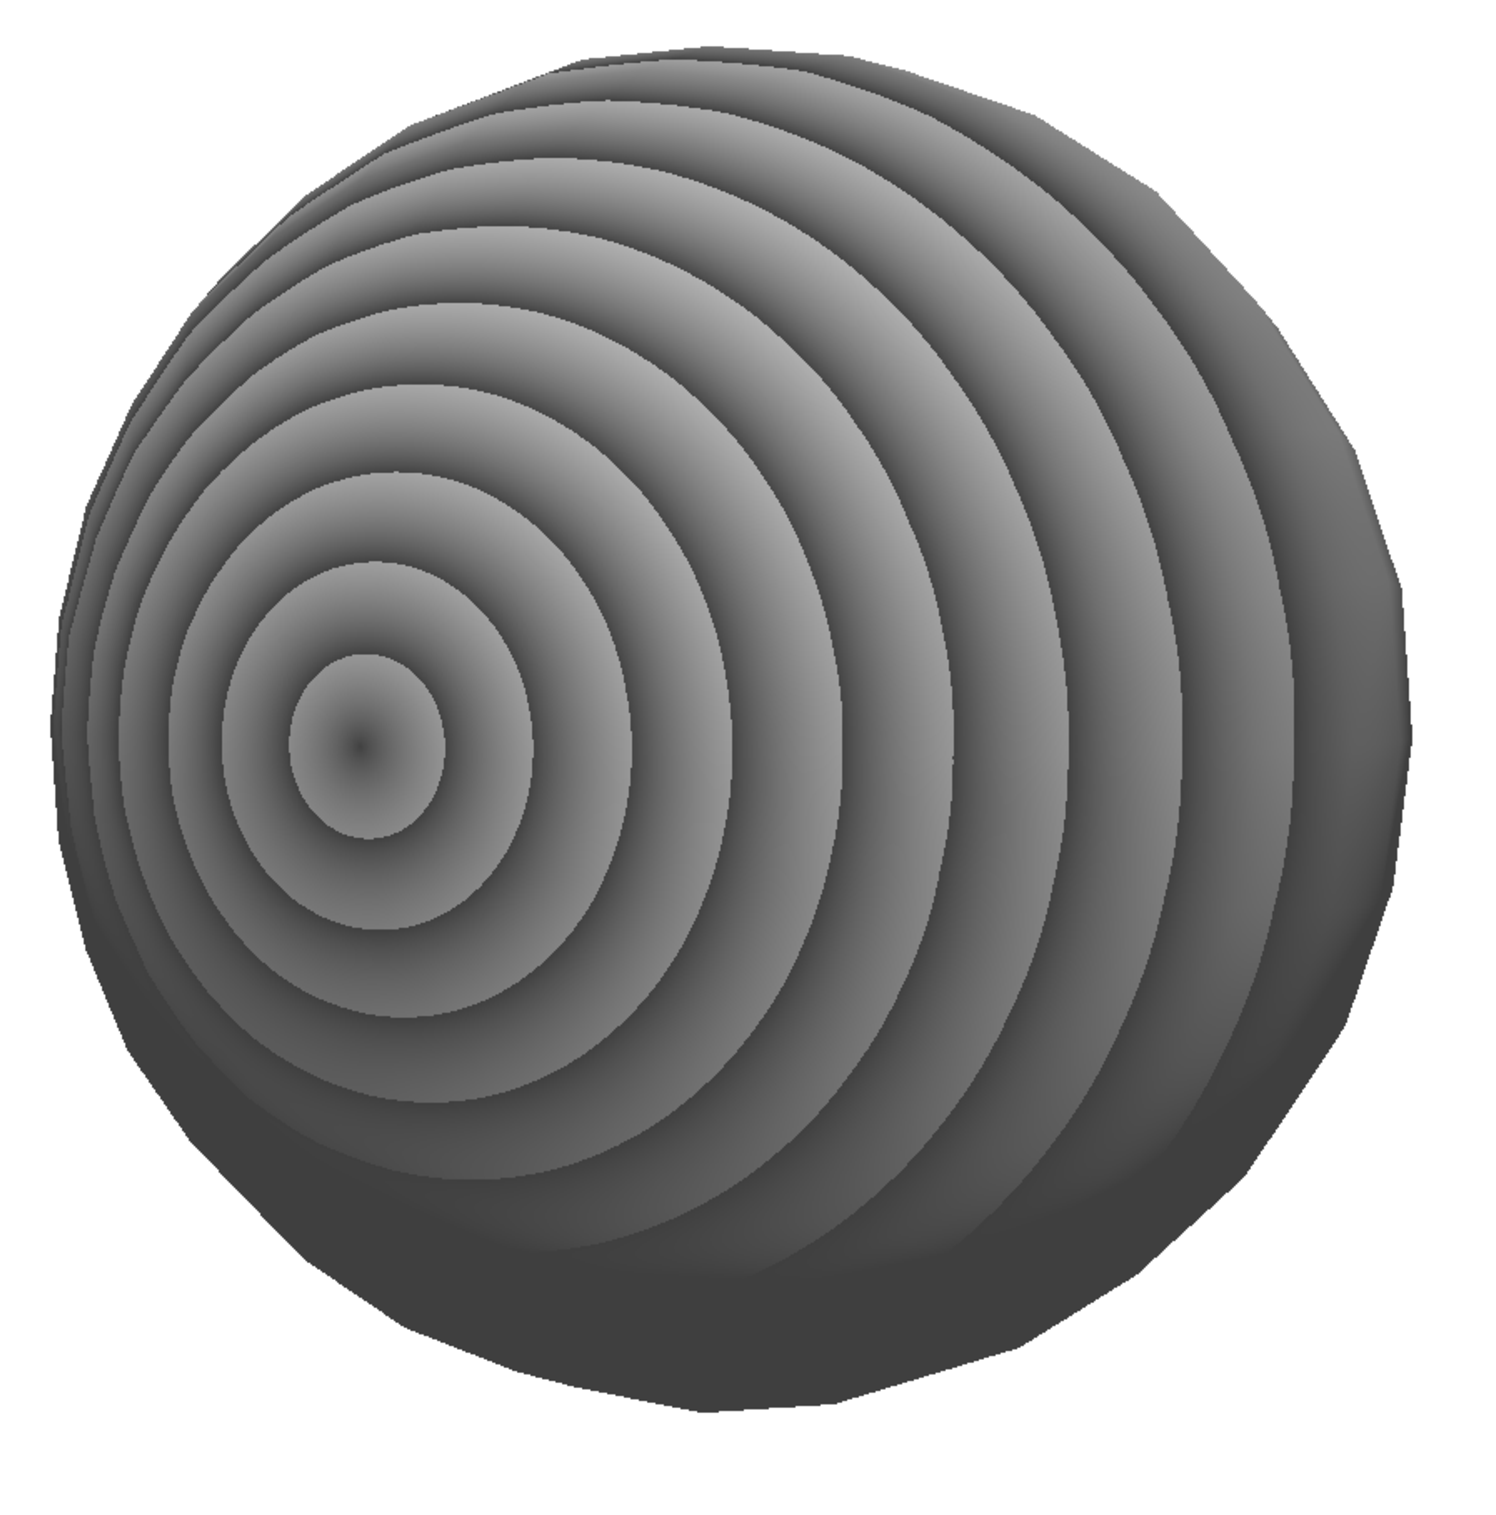
\includegraphics[width=.5\textwidth]{pics/procedural/letokruhy.eps}

  \begin{minted}[frame=lines]{glsl}
float d = length(model_pos.xy);
float t = mod(d*10, 1);
  \end{minted}
\end{frame}

\begin{frame}[fragile]
    \frametitle{Letokruhy obarvíme}
    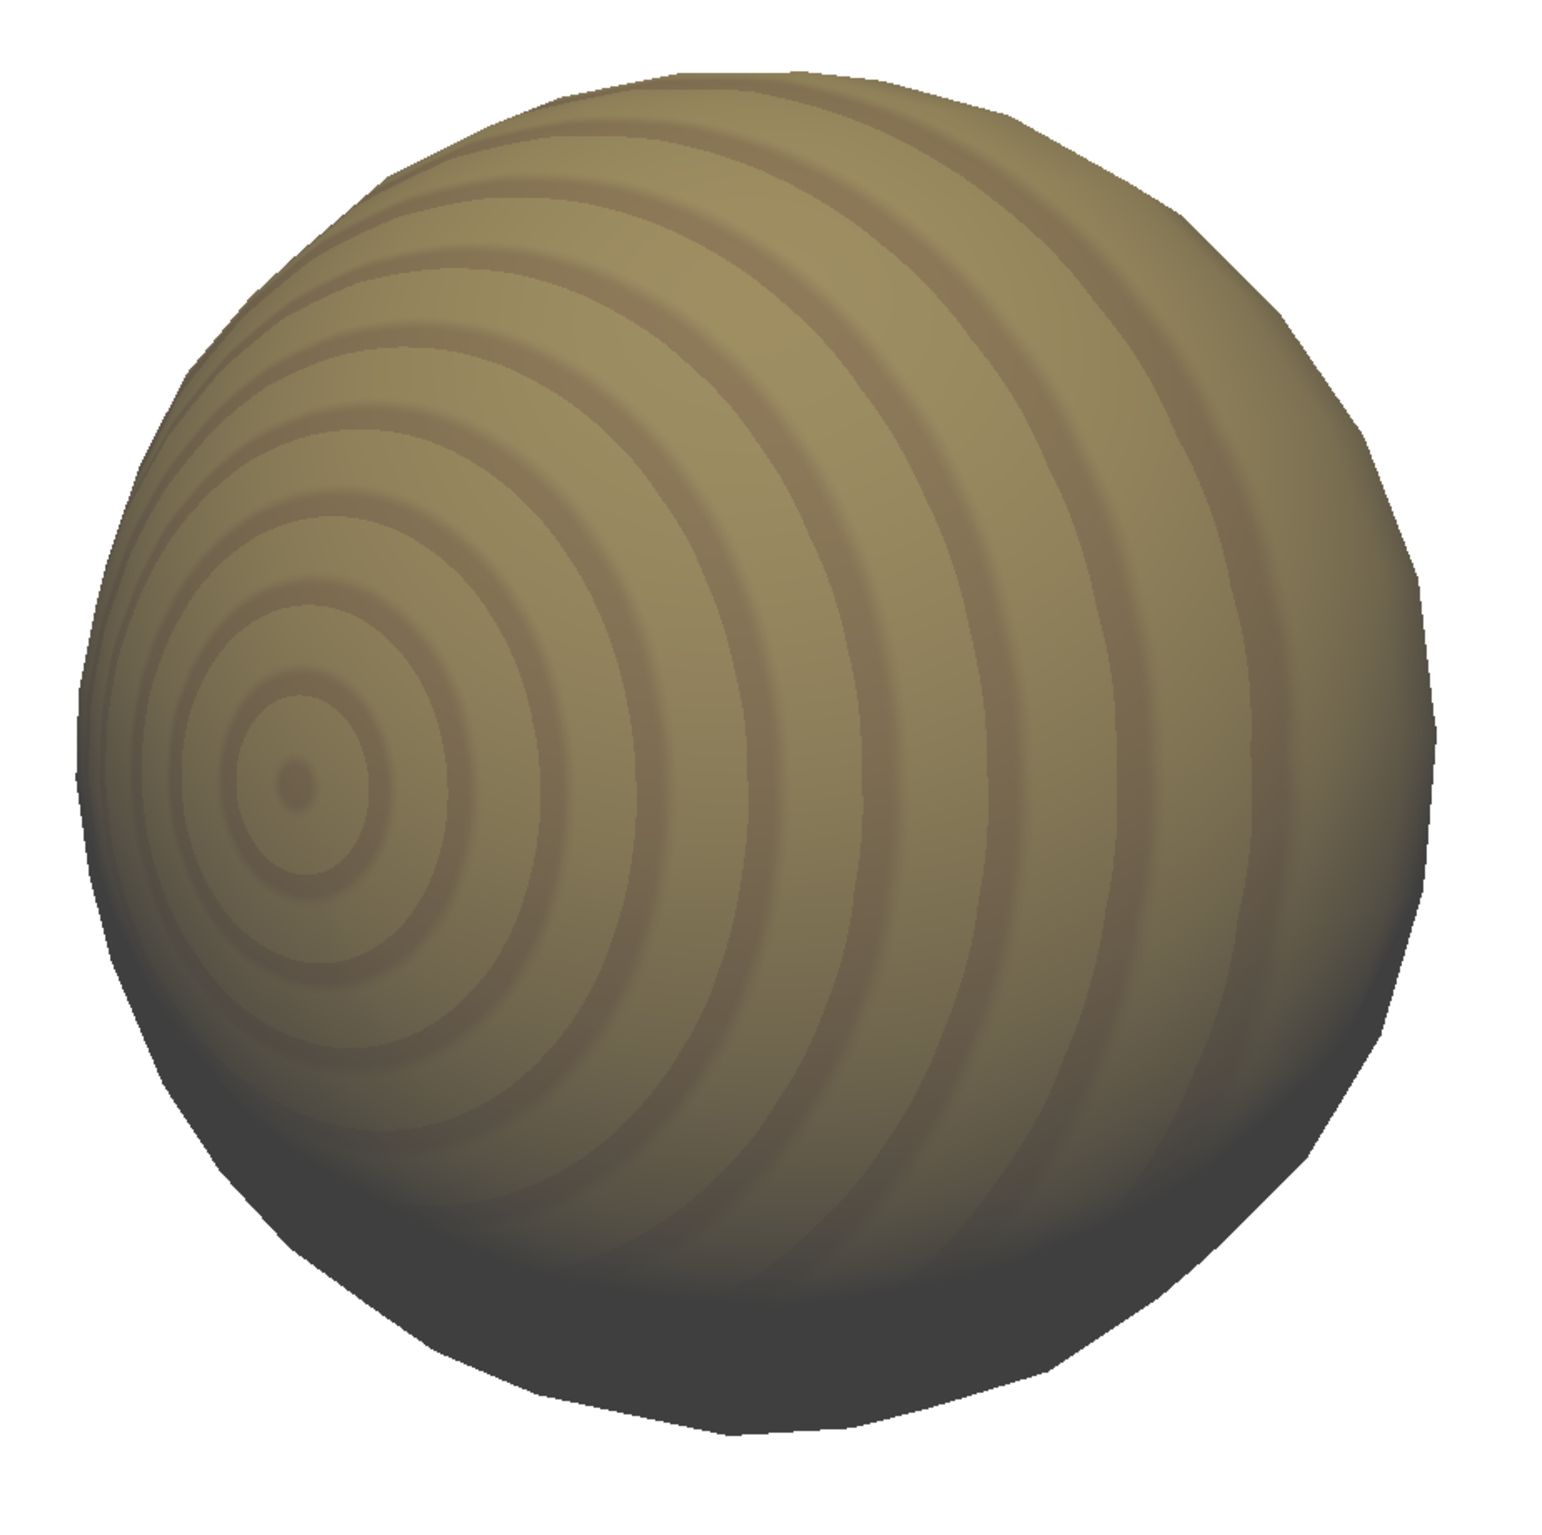
\includegraphics[width=.5\textwidth]{pics/procedural/letokruhy_barva.eps}

  \begin{minted}[frame=lines]{glsl}
vec3 brown = vec3(140, 90, 27)/255;
vec3 yellow = vec3(188, 140, 42)/255;

float t = smoothstep(0.2, 0.4, mod(length(model_pos.xy)*10, 1));
vec3 color = (1-t)*brown + t*yellow;
  \end{minted}
\end{frame}

\begin{frame}[fragile]
    \frametitle{Přidáme šum}
    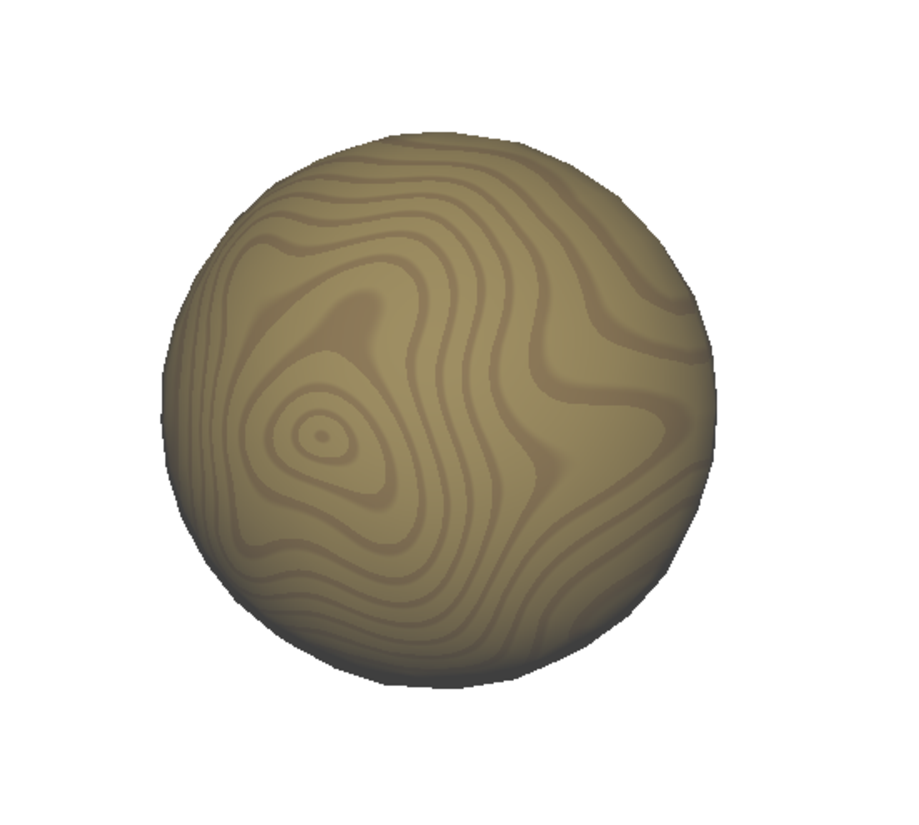
\includegraphics[width=.6\textwidth]{pics/procedural/drevo.eps}

  \begin{minted}[frame=lines]{glsl}
vec2 noisy_pos = model_pos.xy
    + 0.1*fnoise(model_pos.xy);

float t = smoothstep(0.2, 0.4, mod(length(noisy_pos)*10, 1));
vec3 color = (1-t)*brown + t*yellow;
  \end{minted}
\end{frame}

